% Options for packages loaded elsewhere
\PassOptionsToPackage{unicode}{hyperref}
\PassOptionsToPackage{hyphens}{url}
\PassOptionsToPackage{dvipsnames,svgnames,x11names}{xcolor}
%
\documentclass[
  letterpaper,
  DIV=11,
  numbers=noendperiod]{scrartcl}

\usepackage{amsmath,amssymb}
\usepackage{iftex}
\ifPDFTeX
  \usepackage[T1]{fontenc}
  \usepackage[utf8]{inputenc}
  \usepackage{textcomp} % provide euro and other symbols
\else % if luatex or xetex
  \usepackage{unicode-math}
  \defaultfontfeatures{Scale=MatchLowercase}
  \defaultfontfeatures[\rmfamily]{Ligatures=TeX,Scale=1}
\fi
\usepackage{lmodern}
\ifPDFTeX\else  
    % xetex/luatex font selection
\fi
% Use upquote if available, for straight quotes in verbatim environments
\IfFileExists{upquote.sty}{\usepackage{upquote}}{}
\IfFileExists{microtype.sty}{% use microtype if available
  \usepackage[]{microtype}
  \UseMicrotypeSet[protrusion]{basicmath} % disable protrusion for tt fonts
}{}
\makeatletter
\@ifundefined{KOMAClassName}{% if non-KOMA class
  \IfFileExists{parskip.sty}{%
    \usepackage{parskip}
  }{% else
    \setlength{\parindent}{0pt}
    \setlength{\parskip}{6pt plus 2pt minus 1pt}}
}{% if KOMA class
  \KOMAoptions{parskip=half}}
\makeatother
\usepackage{xcolor}
\setlength{\emergencystretch}{3em} % prevent overfull lines
\setcounter{secnumdepth}{-\maxdimen} % remove section numbering
% Make \paragraph and \subparagraph free-standing
\makeatletter
\ifx\paragraph\undefined\else
  \let\oldparagraph\paragraph
  \renewcommand{\paragraph}{
    \@ifstar
      \xxxParagraphStar
      \xxxParagraphNoStar
  }
  \newcommand{\xxxParagraphStar}[1]{\oldparagraph*{#1}\mbox{}}
  \newcommand{\xxxParagraphNoStar}[1]{\oldparagraph{#1}\mbox{}}
\fi
\ifx\subparagraph\undefined\else
  \let\oldsubparagraph\subparagraph
  \renewcommand{\subparagraph}{
    \@ifstar
      \xxxSubParagraphStar
      \xxxSubParagraphNoStar
  }
  \newcommand{\xxxSubParagraphStar}[1]{\oldsubparagraph*{#1}\mbox{}}
  \newcommand{\xxxSubParagraphNoStar}[1]{\oldsubparagraph{#1}\mbox{}}
\fi
\makeatother


\providecommand{\tightlist}{%
  \setlength{\itemsep}{0pt}\setlength{\parskip}{0pt}}\usepackage{longtable,booktabs,array}
\usepackage{calc} % for calculating minipage widths
% Correct order of tables after \paragraph or \subparagraph
\usepackage{etoolbox}
\makeatletter
\patchcmd\longtable{\par}{\if@noskipsec\mbox{}\fi\par}{}{}
\makeatother
% Allow footnotes in longtable head/foot
\IfFileExists{footnotehyper.sty}{\usepackage{footnotehyper}}{\usepackage{footnote}}
\makesavenoteenv{longtable}
\usepackage{graphicx}
\makeatletter
\newsavebox\pandoc@box
\newcommand*\pandocbounded[1]{% scales image to fit in text height/width
  \sbox\pandoc@box{#1}%
  \Gscale@div\@tempa{\textheight}{\dimexpr\ht\pandoc@box+\dp\pandoc@box\relax}%
  \Gscale@div\@tempb{\linewidth}{\wd\pandoc@box}%
  \ifdim\@tempb\p@<\@tempa\p@\let\@tempa\@tempb\fi% select the smaller of both
  \ifdim\@tempa\p@<\p@\scalebox{\@tempa}{\usebox\pandoc@box}%
  \else\usebox{\pandoc@box}%
  \fi%
}
% Set default figure placement to htbp
\def\fps@figure{htbp}
\makeatother
% definitions for citeproc citations
\NewDocumentCommand\citeproctext{}{}
\NewDocumentCommand\citeproc{mm}{%
  \begingroup\def\citeproctext{#2}\cite{#1}\endgroup}
\makeatletter
 % allow citations to break across lines
 \let\@cite@ofmt\@firstofone
 % avoid brackets around text for \cite:
 \def\@biblabel#1{}
 \def\@cite#1#2{{#1\if@tempswa , #2\fi}}
\makeatother
\newlength{\cslhangindent}
\setlength{\cslhangindent}{1.5em}
\newlength{\csllabelwidth}
\setlength{\csllabelwidth}{3em}
\newenvironment{CSLReferences}[2] % #1 hanging-indent, #2 entry-spacing
 {\begin{list}{}{%
  \setlength{\itemindent}{0pt}
  \setlength{\leftmargin}{0pt}
  \setlength{\parsep}{0pt}
  % turn on hanging indent if param 1 is 1
  \ifodd #1
   \setlength{\leftmargin}{\cslhangindent}
   \setlength{\itemindent}{-1\cslhangindent}
  \fi
  % set entry spacing
  \setlength{\itemsep}{#2\baselineskip}}}
 {\end{list}}
\usepackage{calc}
\newcommand{\CSLBlock}[1]{\hfill\break\parbox[t]{\linewidth}{\strut\ignorespaces#1\strut}}
\newcommand{\CSLLeftMargin}[1]{\parbox[t]{\csllabelwidth}{\strut#1\strut}}
\newcommand{\CSLRightInline}[1]{\parbox[t]{\linewidth - \csllabelwidth}{\strut#1\strut}}
\newcommand{\CSLIndent}[1]{\hspace{\cslhangindent}#1}

\KOMAoption{captions}{tablesignature}
\makeatletter
\@ifpackageloaded{caption}{}{\usepackage{caption}}
\AtBeginDocument{%
\ifdefined\contentsname
  \renewcommand*\contentsname{Table of contents}
\else
  \newcommand\contentsname{Table of contents}
\fi
\ifdefined\listfigurename
  \renewcommand*\listfigurename{List of Figures}
\else
  \newcommand\listfigurename{List of Figures}
\fi
\ifdefined\listtablename
  \renewcommand*\listtablename{List of Tables}
\else
  \newcommand\listtablename{List of Tables}
\fi
\ifdefined\figurename
  \renewcommand*\figurename{Figure}
\else
  \newcommand\figurename{Figure}
\fi
\ifdefined\tablename
  \renewcommand*\tablename{Table}
\else
  \newcommand\tablename{Table}
\fi
}
\@ifpackageloaded{float}{}{\usepackage{float}}
\floatstyle{ruled}
\@ifundefined{c@chapter}{\newfloat{codelisting}{h}{lop}}{\newfloat{codelisting}{h}{lop}[chapter]}
\floatname{codelisting}{Listing}
\newcommand*\listoflistings{\listof{codelisting}{List of Listings}}
\makeatother
\makeatletter
\makeatother
\makeatletter
\@ifpackageloaded{caption}{}{\usepackage{caption}}
\@ifpackageloaded{subcaption}{}{\usepackage{subcaption}}
\makeatother

\usepackage{bookmark}

\IfFileExists{xurl.sty}{\usepackage{xurl}}{} % add URL line breaks if available
\urlstyle{same} % disable monospaced font for URLs
\hypersetup{
  pdftitle={Using Cellular Communication Sensing to Support Early Recovery from Alcohol Use Disorder},
  pdfauthor={Kendra Wyant; Coco Yu; John J. Curtin},
  pdfkeywords={Substance use disorders, Machine learning, Cellular
Sensing},
  colorlinks=true,
  linkcolor={blue},
  filecolor={Maroon},
  citecolor={Blue},
  urlcolor={Blue},
  pdfcreator={LaTeX via pandoc}}


\title{Using Cellular Communication Sensing to Support Early Recovery
from Alcohol Use Disorder}
\author{Kendra Wyant \and Coco Yu \and John J. Curtin}
\date{2025-10-02}

\begin{document}
\maketitle


\section{Introduction}\label{introduction}

One of the biggest challenges in Alcohol Use Disorders (AUD) treatment
stems from the chronic relapsing nature of this disease (Scott et al.,
2005). People can relapse days, weeks, and even years after obtaining
the goal of abstinence. At least 60\% of AUD patients relapse to heavy
drinking within 6 months following treatment (Kirshenbaum et al., 2009;
Nguyen et al., 2020; Witkiewitz, 2011). At most 50\% of people with an
AUD achieve remission after several years (Fleury et al., 2016; Heyman,
2013).

Identifying initial lapses in early recovery is critical. Lapses --
single episodes of alcohol use -- are easy to define, have a clear
onset, and are also clinically meaningful. They serve as an early
warning sign of returning back to previous drinking behavior
inconsistent with desired goals (Chung \& Maisto, 2006; Marlatt \&
Donovan, 2005; \textbf{witkiewitzRelapsePreventionAlcohol2004b?}). Lapse
predicts future lapses, with more frequent ones resulting in increased
risks of relapse (Högström Brandt et al., 1999;
\textbf{witkiewitzRelapsePreventionAlcohol2004?}).

Current predictions of alcohol lapses rely heavily on self reports,
which can be burdensome to measure in long run. Machine learning models
leveraging ecological momentary assessment (EMA) measures have performed
relatively well to predict goal-inconsistent alcohol use (Wyant et al.,
2024). The surveys were collected up to four times daily for three
months. However, constantly completing surveys makes it burdensome for
AUD patients. Although most EMA relevant mental health research
demonstrated modest compliance rates, their time windows last from two
weeks to three months (Czyz et al., 2018; Hung et al., 2016;
Mackesy-Amiti \& Boodram, 2018; Porras-Segovia et al., 2020; van
Genugten et al., 2020). The study length is insufficient because AUD is
a chronic disease that requires constant risk monitoring. As extended
period of time is anticipated, users' perceived burden of answering
surveys is presumably larger (Mogk et al., 2023). Although minimizing
the number of items in the surveys and the frequency of prompting users
to complete the surveys might help mitigate the associated burden, it
can inevitably reduce the prediction precision and temporal precision of
predictions.

Passive cellular communication sensing represents new opportunities due
to its feasibility, relatively low burden on individuals and continuous
data collection. In a smartphone-based sensing platform the primary
expense on the individual is the smartphone. Smartphone usage is already
widespread. Eighty-five percent of US adults have a smartphone and this
number is consistent across all sociodemographic groups, including those
in recovery programs for substance use (Center, 2021; Masson et al.,
2019). Studies collecting passive data have demonstrated high
acceptability from participants and higher compliance rates compared to
active measures (Beukenhorst et al., 2022; Wyant et al., 2023). Further,
risk monitoring using cellular sensing is temporally sensitive to
fluctuating risks. Analyzing communication patterns can detect potential
triggers in time without actively prompting users to reflect on their
feelings at the moment or report their environment.

Cellular communications, with minimal contextual information, is
embedded with potentially rich information that align with relapse
antecedents. For example, social interactions can have important
influences on drinking behavior (Alvarez et al., 2021; Hunter-Reel et
al., 2009). We may be able to capture immediate risk based on who
someone is calling or what time of day it is. Decreased interactions may
signify isolation common with depressive symptoms, reaching out to
people in one's social network could signify a positive coping strategy,
or changes in patterns between a single person in one's social network
could indicate conflict (Chih et al., 2014; Hufford et al., 2003; Miller
et al., 2001).

This study aims at building machine learning models from cellular
communications that identify \emph{who} are at heightened risk for
alcohol lapses, \emph{when} they will lapse, and \emph{why} they are at
increased risk.

\section{Methods}\label{methods}

\subsection{Transparency and Openness}\label{transparency-and-openness}

We adhere to research transparency principles that are crucial for
robust and replicable science. We reported how we determined the sample
size, all data exclusions, all manipulations, and all study measures. We
provide a transparency report in the supplement (Aczel et al., 2019).
Our data, questionnaires, and other study materials are publicly
available on our OSF page (\url{https://osf.io/wgpz9/}). Our annotated
analysis scripts and results are publicly available on our study website
(\url{https://jjcurtin.github.io/study_messages/}).

\subsection{Participants}\label{participants}

We recruited 192 participants in early recovery from AUD in Madison,
Wisconsin, USA via print and targeted digital advertisements and
partnerships with treatment centers. This sample size was determined
based on traditional power analysis methods for logistic regression
(Hsieh, 1989). We required that participants:

\begin{enumerate}
\def\labelenumi{\arabic{enumi}.}
\tightlist
\item
  were age 18 or older,
\item
  could write and read in English,
\item
  had at least moderate AUD (\textgreater= 4 self-reported DSM-5
  symptoms),
\item
  were abstinent from alcohol for 1-8 weeks, and
\item
  were willing to use a single smartphone (personal or study provided)
  while on study.
\item
  were not exhibiting severe symptoms of psychosis or
  paranoia.\footnote{Defined as scores \textgreater2.2 or 2.8,
    respectively, on the psychosis or paranoia scales of the Symptom
    Checklist--90 (Derogatis, L.R., 2000)}
\end{enumerate}

One hundred sixty-nine participants were eligible and enrolled in the
study. Fifteen participants discontinued before the first monthly
follow-up visit. We excluded data from one participant who did not
maintain a goal of abstinence during their participation. We also
excluded data from two participants due to evidence of careless
responding and unusually low compliance. Our final sample consisted of
151 participants.

\subsection{Procedure}\label{procedure}

All procedures were approved by the University of Wisconsin-Madison
Institutional Review Board (Study \#2015-0780). Participants completed 5
study visits over approximately 3 months. Participants attended an
in-person screening visit where we determined eligibility, obtained
informed consent, and administered a battery of self-report measures.
Eligible, consented participants returned approximately 1 week later for
an intake visit. Three additional follow-up visits occurred about every
30 days that participants remained on study. At each follow-up visit, we
downloaded participants' voice call and SMS text message logs from their
smartphone devices, collected contextual self-report information about
important contacts, and administered additional self-report measures.

Participants were expected to complete 4 brief (7-10 questions) daily
ecological momentary assessments (EMA) for the duration of their
enrollment. The first item on each EMA asked participants to report
dates and times of any recent alcohol use. At follow-up visits, we
verified lapse reports and queried participants about additional
unreported laspes using a timeline followback measure. Additional
sensing data streams (geolocation, sleep quality, and audio check-ins)
were collected as part of the parent grant's aims (R01 AA024391).

\subsection{Measures}\label{measures}

\subsection{Cellular Communication
Logs}\label{cellular-communication-logs}

\subsection{Context}\label{context}

Participants were asked contextual questions about important contacts
(people whom the partcipant communicated with at least twice by voice
call or SMS text message in a one month period).

\subsection{Data Analysis Plan}\label{data-analysis-plan}

\subsubsection{Model Configurations}\label{model-configurations}

\subsubsection{Feature Engineering}\label{feature-engineering}

\subsubsection{Model Evaluation}\label{model-evaluation}

\subsubsection{Model Comparison}\label{model-comparison}

\subsubsection{Feature Importance}\label{feature-importance}

\section{Results}\label{results}

\subsection{Participants}\label{participants-1}

\subsection{Model Evaluation}\label{model-evaluation-1}

\subsection{Model Comparison}\label{model-comparison-1}

\subsection{Feature Importance}\label{feature-importance-1}

\begin{figure}[H]

\centering{

\pandocbounded{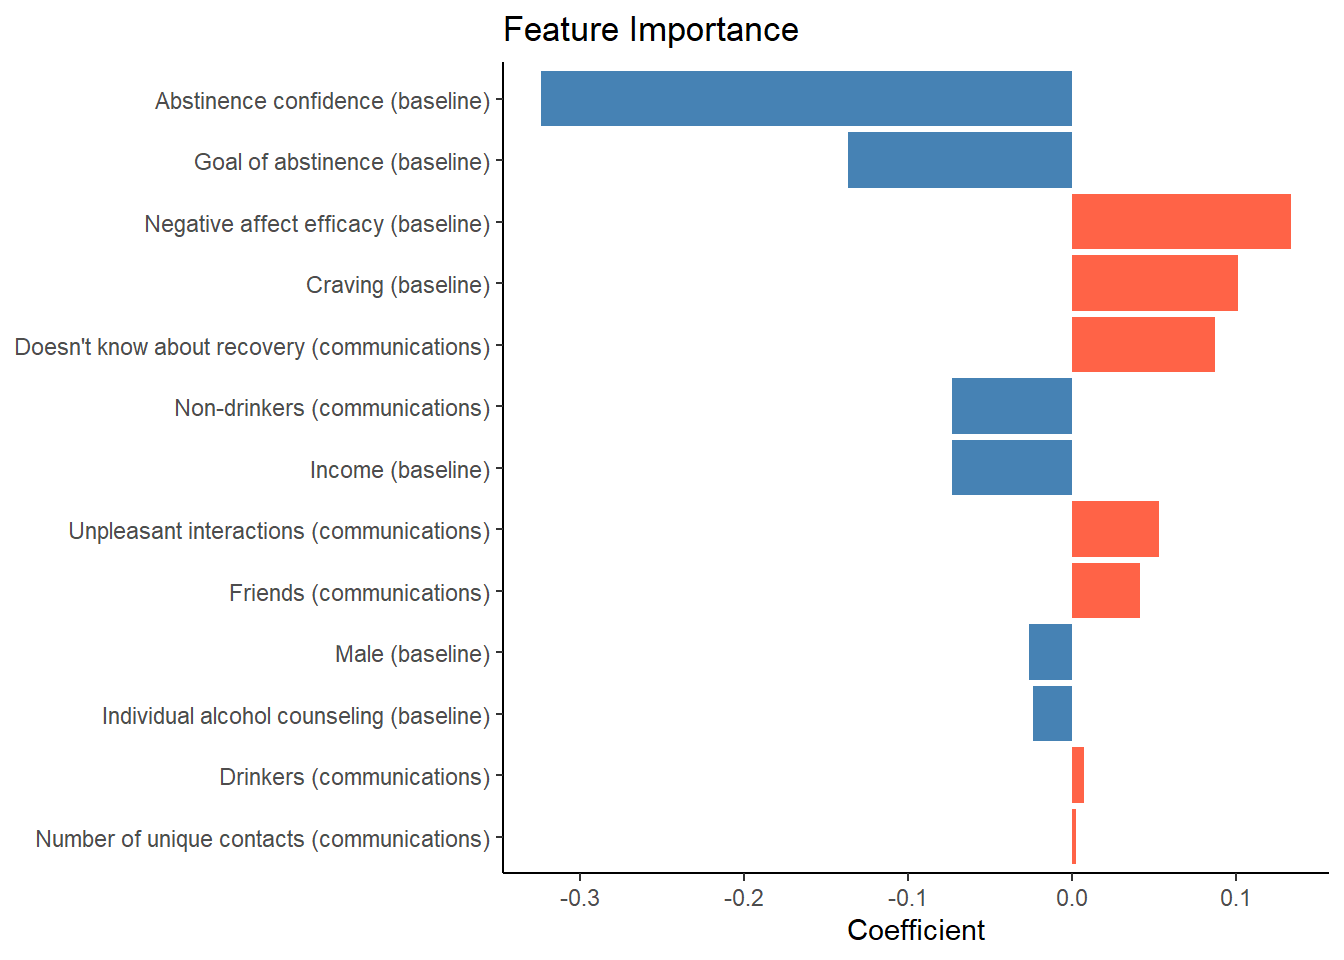
\includegraphics[keepaspectratio]{index_files/figure-latex/notebooks-mak_figures-fig-1-output-1.png}}

}

\caption{\label{fig-1}Global feature importance (glmnet coefficient) for
the full model. Features are ordered by absolute coefficient value. Rate
counts of communications with friends, non-drinkers, and drinkers were
calculated across varying scoring epochs. Standardized coefficients were
averaged across retained epochs to produce single aggregate feature
importance score. Blue bars indicate higher feature values on average
lower lapse risk. Red bars indicate higher feature values on average
increase risk.}

\end{figure}%

\textsubscript{Source:
\href{https://jjcurtin.github.io/study_messages/notebooks/mak_figures-preview.html\#cell-fig-1}{Make
All Figures for Main Manuscript}}

\section{Discussion}\label{discussion}

\newpage

\phantomsection\label{refs}
\begin{CSLReferences}{1}{0}
\bibitem[\citeproctext]{ref-aczelConsensusbasedTransparencyChecklist2019}
Aczel, B., Szaszi, B., Sarafoglou, A., Kekecs, Z., Kucharský, Š.,
Benjamin, D., Chambers, C. D., Fisher, A., Gelman, A., Gernsbacher, M.
A., Ioannidis, J. P., Johnson, E., Jonas, K., Kousta, S., Lilienfeld, S.
O., Lindsay, D. S., Morey, C. C., Monafò, M., Newell, B. R., \ldots{}
Wagenmakers, E.-J. (2019). A consensus-based transparency checklist.
\emph{Nature Human Behaviour}, 1--3.
\url{https://doi.org/10.1038/s41562-019-0772-6}

\bibitem[\citeproctext]{ref-alvarezSocialNetworkHeavy2021a}
Alvarez, M. J., Richards, D. K., Oviedo Ramirez, S., \& Field, C. A.
(2021). Social network heavy drinking moderates the effects of a brief
motivational intervention for alcohol use among injured patients.
\emph{Addictive Behaviors}, \emph{112}, 106594.
\url{https://doi.org/10.1016/j.addbeh.2020.106594}

\bibitem[\citeproctext]{ref-beukenhorstUsingSmartphonesReduce2022a}
Beukenhorst, A. L., Burke, K. M., Scheier, Z., Miller, T. M., Paganoni,
S., Keegan, M., Collins, E., Connaghan, K. P., Tay, A., Chan, J., Berry,
J. D., \& Onnela, J.-P. (2022). Using smartphones to reduce research
burden in a neurodegenerative population and assessing participant
adherence: {A} randomized clinical trial and two observational studies.
\emph{JMIR Mhealth and Uhealth}, \emph{10}(2), e31877.
\url{https://doi.org/10.2196/31877}

\bibitem[\citeproctext]{ref-pewresearchcenterMobileFactSheet2021a}
Center, P. R. (2021). \emph{Mobile {Fact Sheet}}. Pew Research Center.

\bibitem[\citeproctext]{ref-chihPredictiveModelingAddiction2014a}
Chih, M.-Y., Patton, T., McTavish, F. M., Isham, A. J., Judkins-Fisher,
C. L., Atwood, A. K., \& Gustafson, D. H. (2014). Predictive modeling of
addiction lapses in a mobile health application. \emph{Journal of
Substance Abuse Treatment}, \emph{46}(1), 29--35.
\url{https://doi.org/10.1016/j.jsat.2013.08.004}

\bibitem[\citeproctext]{ref-chungRelapseAlcoholOther2006a}
Chung, T., \& Maisto, S. A. (2006). Relapse to alcohol and other drug
use in treated adolescents: {Review} and reconsideration of relapse as a
change point in clinical course. \emph{Clinical Psychology Review},
\emph{26}(2), 149--161. \url{https://doi.org/10.1016/j.cpr.2005.11.004}

\bibitem[\citeproctext]{ref-czyzEcologicalAssessmentDaily2018}
Czyz, E. K., King, C. A., \& Nahum-Shani, I. (2018). Ecological
assessment of daily suicidal thoughts and attempts among suicidal teens
after psychiatric hospitalization: {Lessons} about feasibility and
acceptability. \emph{Psychiatry Research}, \emph{267}, 566--574.
\url{https://doi.org/10.1016/j.psychres.2018.06.031}

\bibitem[\citeproctext]{ref-derogatislBriefSymptomInventory}
Derogatis, L.R. (2000). \emph{Brief {Symptom Inventory} 18 -
{Administration}, scoring, and procedures manual}. NCS Pearson.

\bibitem[\citeproctext]{ref-fleuryRemissionSubstanceUse2016}
Fleury, M.-J., Djouini, A., Huỳnh, C., Tremblay, J., Ferland, F.,
Ménard, J.-M., \& Belleville, G. (2016). Remission from substance use
disorders: {A} systematic review and meta-analysis. \emph{Drug and
Alcohol Dependence}, \emph{168}, 293--306.
\url{https://doi.org/10.1016/j.drugalcdep.2016.08.625}

\bibitem[\citeproctext]{ref-heymanQuittingDrugsQuantitative2013}
Heyman, G. M. (2013). Quitting {Drugs}: {Quantitative} and {Qualitative
Features}. \emph{Annual Review of Clinical Psychology}, \emph{9}(Volume
9, 2013), 29--59.
\url{https://doi.org/10.1146/annurev-clinpsy-032511-143041}

\bibitem[\citeproctext]{ref-hogstrombrandtPredictionSingleEpisodes1999a}
Högström Brandt, A. M., Thorburn, D., Hiltunen, A. J., \& Borg, S.
(1999). Prediction of single episodes of drinking during the treatment
of alcohol-dependent patients. \emph{Alcohol (Fayetteville, N.Y.)},
\emph{18}(1), 35--42.
\url{https://doi.org/10.1016/s0741-8329(98)00065-2}

\bibitem[\citeproctext]{ref-hsiehSampleSizeTables1989}
Hsieh, F. (1989). Sample size tables for logistic regression.
\emph{Statistics in Medicine}, \emph{8}, 795--802.

\bibitem[\citeproctext]{ref-huffordRelapseNonlinearDynamic2003a}
Hufford, M. R., Witkiewitz, K., Shields, A. L., Kodya, S., \& Caruso, J.
C. (2003). Relapse as a nonlinear dynamic system: {Application} to
patients with alcohol use disorders. \emph{Journal of Abnormal
Psychology}, \emph{112}(2), 219--227.
\url{https://doi.org/10.1037/0021-843X.112.2.219}

\bibitem[\citeproctext]{ref-hungSmartphonebasedEcologicalMomentary2016}
Hung, S., Li, M.-S., Chen, Y.-L., Chiang, J.-H., Chen, Y.-Y., \& Hung,
G. C.-L. (2016). Smartphone-based ecological momentary assessment for
{Chinese} patients with depression: {An} exploratory study in {Taiwan}.
\emph{Asian Journal of Psychiatry}, \emph{23}, 131--136.
\url{https://doi.org/10.1016/j.ajp.2016.08.003}

\bibitem[\citeproctext]{ref-hunter-reelEmphasizingInterpersonalFactors2009a}
Hunter-Reel, D., McCrady, B., \& Hildebrandt, T. (2009). Emphasizing
interpersonal factors: {An} extension of the {Witkiewitz} and {Marlatt}
relapse model. \emph{Addiction (Abingdon, England)}, \emph{104}(8),
1281--1290. \url{https://doi.org/10.1111/j.1360-0443.2009.02611.x}

\bibitem[\citeproctext]{ref-kirshenbaumQuantitativeReviewUbiquitous2009}
Kirshenbaum, A. P., Olsen, D. M., \& Bickel, W. K. (2009). A
quantitative review of the ubiquitous relapse curve. \emph{Journal of
Substance Abuse Treatment}, \emph{36}(1), 8--17.
\url{https://doi.org/10.1016/j.jsat.2008.04.001}

\bibitem[\citeproctext]{ref-mackesy-amitiFeasibilityEcologicalMomentary2018}
Mackesy-Amiti, M. E., \& Boodram, B. (2018). Feasibility of ecological
momentary assessment to study mood and risk behavior among young people
who inject drugs. \emph{Drug and Alcohol Dependence}, \emph{187},
227--235. \url{https://doi.org/10.1016/j.drugalcdep.2018.03.016}

\bibitem[\citeproctext]{ref-marlattRelapsePreventionMaintenance2005a}
Marlatt, G. A., \& Donovan, D. M. (Eds.). (2005). \emph{Relapse
prevention: {Maintenance} strategies in the treatment of addictive
behaviors, 2nd ed} (pp. xiv, 416). The Guilford Press.

\bibitem[\citeproctext]{ref-massonHealthrelatedInternetUse2019a}
Masson, C. L., Chen, I. Q., Levine, J. A., Shopshire, M. S., \&
Sorensen, J. L. (2019). Health-related internet use among opioid
treatment patients. \emph{Addictive Behaviors Reports}, \emph{9},
100157. \url{https://doi.org/10.1016/j.abrep.2018.100157}

\bibitem[\citeproctext]{ref-millerHowEffectiveAlcoholism2001a}
Miller, W. R., Walters, S. T., \& Bennett, M. E. (2001). How effective
is alcoholism treatment in the {United States}? \emph{Journal of Studies
on Alcohol}, \emph{62}(2), 211--220.
\url{https://doi.org/10.15288/jsa.2001.62.211}

\bibitem[\citeproctext]{ref-mogkImplementationWorkflowStrategies2023}
Mogk, J. M., Matson, T. E., Caldeiro, R. M., Garza Mcwethy, A. M.,
Beatty, T., Sevey, B. C., Hsu, C. W., \& Glass, J. E. (2023).
Implementation and workflow strategies for integrating digital
therapeutics for alcohol use disorders into primary care: {A}
qualitative study. \emph{Addiction Science \& Clinical Practice},
\emph{18}(1). \url{https://doi.org/10.1186/s13722-023-00387-w}

\bibitem[\citeproctext]{ref-nguyenPredictingRelapseAlcohol2020a}
Nguyen, L.-C., Durazzo, T. C., Dwyer, C. L., Rauch, A. A., Humphreys,
K., Williams, L. M., \& Padula, C. B. (2020). Predicting {Relapse After
Alcohol Use Disorder Treatment} in a {High-Risk Cohort}: {The Roles} of
{Anhedonia} and {Smoking}. \emph{Journal of Psychiatric Research},
\emph{126}, 1--7. \url{https://doi.org/10.1016/j.jpsychires.2020.04.003}

\bibitem[\citeproctext]{ref-porras-segoviaSmartphonebasedEcologicalMomentary2020}
Porras-Segovia, A., Molina-Madueño, R. M., Berrouiguet, S.,
López-Castroman, J., Barrigón, M. L., Pérez-Rodríguez, M. S., Marco, J.
H., Díaz-Oliván, I., de León, S., Courtet, P., Artés-Rodríguez, A., \&
Baca-García, E. (2020). Smartphone-based ecological momentary assessment
({EMA}) in psychiatric patients and student controls: {A} real-world
feasibility study. \emph{Journal of Affective Disorders}, \emph{274},
733--741. \url{https://doi.org/10.1016/j.jad.2020.05.067}

\bibitem[\citeproctext]{ref-scottPathwaysRelapseTreatment2005}
Scott, C. K., Foss, M. A., \& Dennis, M. L. (2005). Pathways in the
relapse--treatment--recovery cycle over 3 years. \emph{Journal of
Substance Abuse Treatment}, \emph{28 Suppl 1}, S63--72.
\url{https://doi.org/10.1016/j.jsat.2004.09.006}

\bibitem[\citeproctext]{ref-vangenugtenExperiencedBurdenAdherence2020}
van Genugten, C. R., Schuurmans, J., Lamers, F., Riese, H., Penninx, B.
W. J. H., Schoevers, R. A., Riper, H. M., \& Smit, J. H. (2020).
Experienced {Burden} of and {Adherence} to {Smartphone-Based Ecological
Momentary Assessment} in {Persons} with {Affective Disorders}.
\emph{Journal of Clinical Medicine}, \emph{9}(2), 322.
\url{https://doi.org/10.3390/jcm9020322}

\bibitem[\citeproctext]{ref-witkiewitzPredictorsHeavyDrinking2011a}
Witkiewitz, K. (2011). Predictors of {Heavy Drinking During} and
{Following Treatment}. \emph{Psychology of Addictive Behaviors : Journal
of the Society of Psychologists in Addictive Behaviors}, \emph{25}(3),
426--438. \url{https://doi.org/10.1037/a0022889}

\bibitem[\citeproctext]{ref-wyantAcceptabilityPersonalSensing2023a}
Wyant, K., Moshontz, H., Ward, S. B., Fronk, G. E., \& Curtin, J. J.
(2023). Acceptability of {Personal Sensing Among People With Alcohol Use
Disorder}: {Observational Study}. \emph{JMIR mHealth and uHealth},
\emph{11}, e41833. \url{https://doi.org/10.2196/41833}

\bibitem[\citeproctext]{ref-wyantMachineLearningModels2024}
Wyant, K., Sant'Ana, S. J., Fronk, G. E., \& Curtin, J. J. (2024).
Machine learning models for temporally precise lapse prediction in
alcohol use disorder. \emph{Journal of Psychopathology and Clinical
Science}, \emph{133}(7), 527--540.
\url{https://doi.org/10.1037/abn0000901}

\end{CSLReferences}




\end{document}
